\section{Manipulation}\label{sec: distance cost}

In this and next section, we consider the cost function $\cost$ induced by the Euclidean distance. For any two attributes $\firstfeatures, \secondfeatures$, we have $\onecost(\firstfeatures,\secondfeatures) = \eta\cdot \|\firstfeatures - \secondfeatures\|_2$, where $\eta>0$ and $\| \cdot \|_2$ is the $\ell^2$ norm. It is without loss of generality to assume that $\eta=1$, which implies that $\onecost(\firstfeatures,\secondfeatures)$ is just the Euclidean distance between $\firstfeatures$ and $\secondfeatures$. We also assume the cost is additive, which means for a path with three attributes $\orifeatures, \firstfeatures, \secondfeatures$, we have 
$\cost(\orifeatures,\firstfeatures,\secondfeatures) = \onecost(\orifeatures,\firstfeatures)+\onecost(\firstfeatures,\secondfeatures) $.


% \subsection{Manipulation}\label{subsec: distance manipulation}
In this section, we focus on the manipulation setting.

\subsection{Optimal sequential mechanism}\label{subsec:seq manipulation}
First consider the scenario where the principal has to  conduct one test at a time.
That is, she is constrained to use sequential mechanisms.
Suppose also that tests cannot be tailored for each agent, i.e., cheap-talk communication is not possible.
Our first theorem answers the question: What is the optimal sequential mechanism? 

\begin{theorem}\label{thm: optimal max qualified}
Suppose $M=\nullset$. 
% Consider the manipulation setting.
    % Suppose the cost is induced by the Euclidean distance and is additive. 
    % Suppose the qualified region is the intersection of two linear classifiers $\classifier_A \cap \classifier_B$.
   For any distribution $\dist$, the optimal sequential mechanism uses
    \begin{enumerate}
        \item  \emph{stringent} tests $\tilde \classifier_A$ and $\tilde \classifier_B$, such that $\tilde\classifier_A \cap \tilde \classifier_B \subset \classifier_A \cap \classifier_B$;
        % uses \emph{stringent} tests, i.e., it announce two tests $\tilde \classifier_A$ and $\tilde \classifier_B$ such that the attributes that pass two tests are in a strict subset of the qualified region $\tilde\classifier_A \cap \tilde \classifier_B \subset \classifier_A \cap \classifier_B$;
        \item a fixed-order procedure.
    \end{enumerate}
\end{theorem}

We call a test that is stricter than the true criterion a stringent test.
    When the agent's type is one-dimensional, there is no room for the design of testing procedure, and the notion of stringent test is a raised threshold \citep{perez2022test}.  When the agent's type is two-dimensional, the first property in \cref{thm: optimal max qualified} points out that the correct notion of stringent tests is $\tilde\classifier_A \cap \tilde \classifier_B \subset \classifier_A \cap \classifier_B$.\footnote{One might conjecture that stringent tests are two shifted parallel tests, i.e.,  $\tilde\classifier_i  \subset \classifier_i$ for $i\in \{A,B\}$. However, \cref{fig:cheap-talk} provides an example on why shifted parallel tests might not be always optimal. Depending on the distribution, the gain from using non-parallel tests could sometimes offset its loss in terms of selecting qualified agents.}
    The second property in \cref{thm: optimal max qualified} is our key innovation. It highlights that when using multiple tests to screen an agent with multi-dimensional  types, the choice of testing procedure is non-trivial: offering the tests sequentially in a fixed-order is (sometimes strictly) better than other procedures.

    \begin{figure}
    \centering
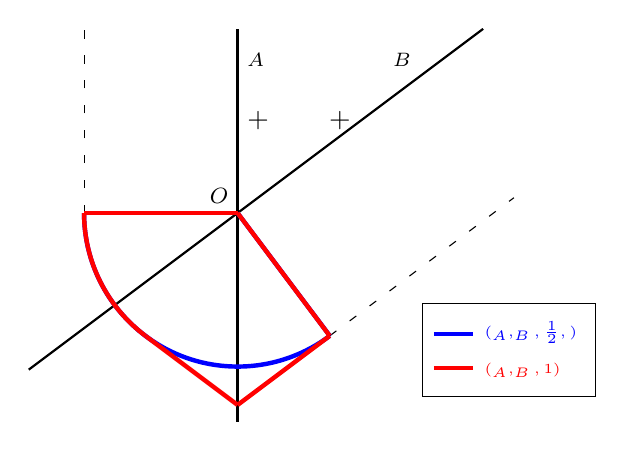
\begin{tikzpicture}[xscale=7.8,yscale=7.8,
    pics/legend entry/.style={code={%   
        \draw[pic actions] 
        (-0.25,0.25) -- (0.25,0.25);}}]


\draw [domain=0.66:1.4, thick] plot (\x, {3/4*\x+1/4});
\node [left] at (1.3, 1.25 ) {$\classifier_B$};%:\feature_2\geq \frac34 \feature_1 +\frac14
\draw [thick] (1,0.66) -- (1,1.3);
\node [right] at (1, 1.25) {$\classifier_A$};%: \feature_1 \geq 1$
\node [above,font=\tiny] at (0.97, 1 ) {\footnotesize$O$};
\node [left] at (1.2,1.15) {$+$};
\node [right] at (1, 1.15) {$+$};

\draw [domain=1+0.25*0.6:1.45, loosely dashed] plot (\x, {3/4*\x+1/4-5/16}); % 1/c = 1/4

\draw [loosely dashed] (1-0.25,1) -- (1-0.25,1.3);


\draw[blue, ultra thick] (1-0.25,1) arc (180:360-53.1:0.25);
\draw[blue, ultra thick] (1,1) -- ++(180:0.25);
 \draw[blue, ultra thick] (1,1) -- ++(360-53.1:0.25) ;

\draw[red, ultra thick] (1-0.25,1) arc (180:233.1:0.25);
\draw[red, ultra thick] (1,1) -- ++(180:0.25);

\draw [ red, ultra thick] (1,11/16) -- (1-0.25*0.6,1-0.25*0.8);
\draw [red, ultra thick] (1,11/16) -- (1+0.25*0.6,1-0.25*0.8);
\draw [red, ultra thick] (1,1) -- (1+0.25*0.6,1-0.25*0.8);


\matrix [draw, above right] at (1.3,0.7) {
\pic[blue, ultra thick]{legend entry}; &  \node[blue,font=\tiny] {$(\classifier_A,\classifier_B,\frac12,\nullset)$}; \\
  \pic[red, ultra thick]{legend entry}; &  \node[red,font=\tiny] {$(\classifier_A,\classifier_B,1)$}; \\
};
\end{tikzpicture}
\caption{Stringency of procedures: random-order without disclosure vs fixed-order} 
 \rule{0in}{1.2em}$^\dag$\scriptsize In this graph, the two procedures share the same tests $\classifier_A$ and $\classifier_B$. Under the same tests, the set in blue and the set in red highlights the critical difference between the set of types that have profitable strategies to pass both tests under a random-order procedure without disclosure $(\classifier_A,\classifier_B,\frac12,\nullset)$ and that under a fixed-order procedure  $(\classifier_A,\classifier_B,1)$.
\label{fig: random uninformed vs fixed}
\end{figure}

    We call a testing procedure X is more stringent than a testing procedure Y if under the same choice of tests,  the set of types that have profitable strategies to pass both tests is larger (or has higher probability) than that under X than that under Y.  As an example, \cref{fig: random uninformed vs fixed} illustrates that a random-order procedure without disclosure is more stringent than a fixed-order procedure because of the set inclusion relation. This is true in general, regardless of the randomization probability.
    As another example, the left panel of \cref{fig: same graph ran_informed fixed 2} compares a fixed-order procedure and a random-order procedure with disclosure. Although there is no direct set inclusion relation here, we prove that the probability of the set of types that can profitably pass both tests under a random-order procedure with disclosure, i.e., the cost of passing both tests is less than one, is smaller than that under a fixed-order procedure, regardless of the randomization probability.
    Hence, a random-order procedure with disclosure is also more stringent than a fixed-order procedure.
    As a third example, we argue that a random-order procedure without disclosure is more stringent than a random-order procedure with disclosure, for the same randomization probability. Consider  point C  in the left panel of \cref{fig: same graph ran_informed fixed 2}. Since this type already passes test $\classifier_A$, he could just wait in the first round and if he is told that the first test was $\classifier_A$, he could pass the second test with a cost $1$. However, this strategy is not profitable if he does not know the first test.
    So without disclosure, this type does not have a profitable strategy to get selected since pass both tests together has a cost higher than $1$.
    
    Given that the principal can use either stringent tests or stringent testing procedure to screen the agent, the critical question is which combination is optimal. \cref{thm: optimal max qualified} states that the least stringent testing procedure combined with stringent tests are optimal.




\begin{figure}
    \centering
    \begin{subfigure}[b]{0.45\linewidth}
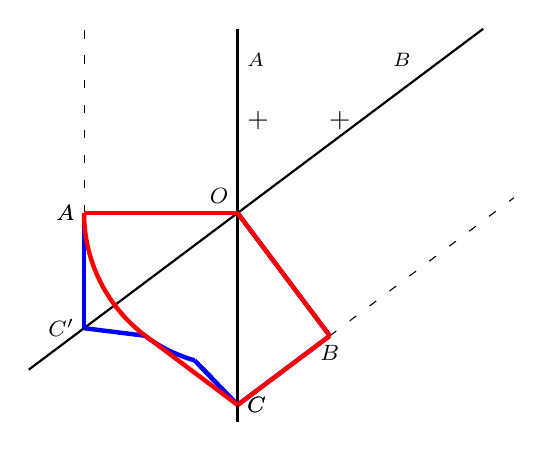
\begin{tikzpicture}[xscale=7.8,yscale=7.8,
    pics/legend entry/.style={code={%   
        \draw[pic actions] 
        (-0.25,0.25) -- (0.25,0.25);}}]

\draw [domain=0.66:1.4, thick] plot (\x, {3/4*\x+1/4});
\node [left] at (1.3, 1.25 ) {$\classifier_B$};%:\feature_2\geq \frac34 \feature_1 +\frac14
\draw [thick] (1,0.66) -- (1,1.3);
\node [right] at (1, 1.25) {$\classifier_A$};%: \feature_1 \geq 1$
\node [above,font=\tiny] at (0.97, 1 ) {\footnotesize$O$};
\node [left] at (1.2,1.15) {$+$};
\node [right] at (1, 1.15) {$+$};


\draw [domain=1+0.25*0.6:1.45, loosely dashed] plot (\x, {3/4*\x+1/4-5/16}); 
\draw [loosely dashed] (1,1) -- (1+0.25*0.6,1-0.25*0.8);

\draw [loosely dashed] (1-0.25,1) -- (1-0.25,1.3);
\draw [loosely dashed] (1-0.25,1) -- (1,1);

\draw [blue, ultra thick] (1-0.25,1) -- (1-0.25,{3/4*0.75+1/4});
\node [left, font=\tiny] at (1-0.25, 1 ) {\footnotesize$A$};

\node [left, font=\tiny] at (1-0.25, {3/4*0.75+1/4} ) {\footnotesize$C'$};


\draw[blue, ultra thick]  (0.93 ,{-1/sqrt(1/0.72^2-1)*(0.93-1)+11/16}) arc (254.1:232.8:0.25);

\draw[blue, ultra thick] (1,1) -- ++(180:0.25);
\draw[ blue, ultra thick] (1,1) -- ++(360-53.1:0.25) ;

\draw [blue, ultra thick] (1,11/16) -- (0.94,{-1/sqrt(1/0.72^2-1)*(0.94-1)+11/16});
\node [right] at (1,11/16) {\footnotesize$C$};
\draw [blue, ultra thick] (1,11/16) -- (1+0.25*0.6,1-0.25*0.8);

\draw [domain=0.93:1, blue, ultra thick] plot (\x, {-1/sqrt(1/0.72^2-1)*(\x-1)+11/16}); 
% \node[below] at (0.93 ,{-1/sqrt(1/0.72^2-1)*(0.93-1)+11/16}) {\footnotesize$D$};

 \draw [domain=1-0.25:0.85, blue, ultra thick] plot (\x, {tan(-7.075621914)*(\x-0.75)+13/16}); 




\draw[red, ultra thick] (1-0.25,1) arc (180:233.1:0.25);
\draw[red, ultra thick] (1,1) -- ++(180:0.25);
\draw [ red, ultra thick] (1,11/16) -- (1-0.25*0.6,1-0.25*0.8);
\draw [red, ultra thick] (1,11/16) -- (1+0.25*0.6,1-0.25*0.8);
\draw [red, ultra thick] (1,1) -- (1+0.25*0.6,1-0.25*0.8);

\node [left, font=\tiny] at (1-0.25, 1 ) {\footnotesize$A$};
\node [below, font=\tiny] at (1+0.25*0.6,1-0.25*0.8) {\footnotesize$B$};
% \node [below, font=\tiny] at (1-0.25*0.6,1-0.25*0.8) {\footnotesize$B'$};
\node [right, font=\tiny] at (1,11/16) {\footnotesize$C$};

\end{tikzpicture}
 \end{subfigure}
\begin{subfigure}[b]{0.45\linewidth}
    \centering
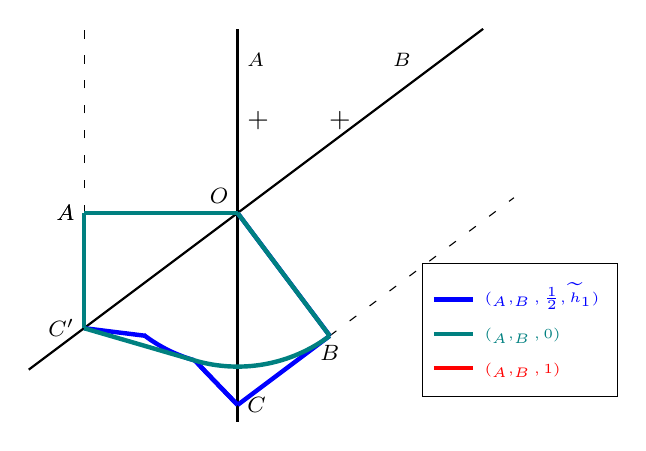
\begin{tikzpicture}[xscale=7.8,yscale=7.8,
    pics/legend entry/.style={code={%   
        \draw[pic actions] 
        (-0.25,0.25) -- (0.25,0.25);}}]

\draw [domain=0.66:1.4, thick] plot (\x, {3/4*\x+1/4});
\node [left] at (1.3, 1.25 ) {$\classifier_B$};%:\feature_2\geq \frac34 \feature_1 +\frac14
\draw [thick] (1,0.66) -- (1,1.3);
\node [right] at (1, 1.25) {$\classifier_A$};%: \feature_1 \geq 1$
\node [above,font=\tiny] at (0.97, 1 ) {\footnotesize$O$};
\node [left] at (1.2,1.15) {$+$};
\node [right] at (1, 1.15) {$+$};


\draw [domain=1+0.25*0.6:1.45, loosely dashed] plot (\x, {3/4*\x+1/4-5/16}); 
\draw [loosely dashed] (1,1) -- (1+0.25*0.6,1-0.25*0.8);

\draw [loosely dashed] (1-0.25,1) -- (1-0.25,1.3);
\draw [loosely dashed] (1-0.25,1) -- (1,1);


\node [left, font=\tiny] at (1-0.25, 1 ) {\footnotesize$A$};

\node [left, font=\tiny] at (1-0.25, {3/4*0.75+1/4} ) {\footnotesize$C'$};

\draw [blue, ultra thick] (1-0.25,1) -- (1-0.25,{3/4*0.75+1/4});
\draw[blue, ultra thick]  (0.93 ,{-1/sqrt(1/0.72^2-1)*(0.93-1)+11/16}) arc (254.1:232.8:0.25);

\draw[blue, ultra thick] (1,1) -- ++(180:0.25);
\draw[ blue, ultra thick] (1,1) -- ++(360-53.1:0.25) ;


\draw [blue, ultra thick] (1,11/16) -- (0.94,{-1/sqrt(1/0.72^2-1)*(0.94-1)+11/16});
\node [right] at (1,11/16) {\footnotesize$C$};
\draw [blue, ultra thick] (1,11/16) -- (1+0.25*0.6,1-0.25*0.8);

\draw [domain=0.93:1, blue, ultra thick] plot (\x, {-1/sqrt(1/0.72^2-1)*(\x-1)+11/16}); 
% \node[below] at (0.93 ,{-1/sqrt(1/0.72^2-1)*(0.93-1)+11/16}) {\footnotesize$D$};

 \draw [domain=1-0.25:0.85, blue, ultra thick] plot (\x, {tan(-7.075621914)*(\x-0.75)+13/16}); 




\draw[teal, ultra thick] (1+0.25*0.6,1-0.25*0.8) arc (360-53.1:360-53.1*2:0.25);
% \draw[red, ultra thick] (1,1) -- ++(360-53.1*2:0.25);


% \draw [ red, ultra thick] (1,11/16) -- (1-0.25*0.6,1-0.25*0.8);
\draw [teal, ultra thick]  (1,1 ) -- (1-0.25, 1 );
\draw [teal, ultra thick]  (1-0.25, {3/4*0.75+1/4} ) -- (1-0.25, 1 );
\draw [teal, ultra thick]  (1-0.25, {3/4*0.75+1/4} ) -- ({1-0.25*sin(106.2-90)},{1-0.25*cos(106.2-90)});
\draw[teal, ultra thick] (1,1) -- (1+0.25*0.6,1-0.25*0.8);

\node [left, font=\tiny] at (1-0.25, 1 ) {\footnotesize$A$};
\node [below, font=\tiny] at (1+0.25*0.6,1-0.25*0.8) {\footnotesize$B$};
% \node [below, font=\tiny] at (1-0.25*0.6,1-0.25*0.8) {\footnotesize$B'$};
% \node [right, font=\tiny] at (1,11/16) {\footnotesize$C$};
\matrix [draw, above right] at (1.3,0.7) {
\pic[blue, ultra thick]{legend entry}; &  \node[blue,font=\tiny] {$(\classifier_A,\classifier_B,\frac12,\widetilde h_1)$}; \\
 \pic[teal, ultra thick]{legend entry}; &  \node[teal,font=\tiny] {$(\classifier_A,\classifier_B,0)$}; \\
  \pic[red, ultra thick]{legend entry}; &  \node[red,font=\tiny] {$(\classifier_A,\classifier_B,1)$}; \\
};
\end{tikzpicture}
 \end{subfigure}
 \caption{Lack of nested structure: random-order procedure with disclosure vs fixed-order procedures}
 \label{fig: same graph ran_informed fixed 2}
\end{figure}

We first provide a tempting but oversimplified intuition.
% In any sequential mechanism,  the agent can pass one test (potentially failing another) at a time.
% Intuitively, fixing the same tests, any random-order mechanism (without disclosure) allows fewer agents to manipulate their types compared to fixed-order mechanism.
% Notice that the way to manipulate one's type to pass one test (that meets one of the principal's criteria) is usually different from that to pass another test (that meets another criteria), especially when the two criteria are in conflict.
% As a result, randomness introduces strategic uncertainty and makes it harder for the agent to predict what is the first test.
To exclude unqualified agents (feasibility), stringent tests must be used regardless of the testing procedure. 
Notice that this also excludes potential qualified agents.
Hence if the same stringent tests are used under all procedures, then a fixed-order mechanism is better than a random-order mechanism, because this former helps more qualified agents to get selected under the stringent tests (see \cref{fig: oversimplified intuition}).
However, this intuition is oversimplified, because the choice of tests usually interacts with the choice of testing procedures.
While the fixed-order procedure helps qualified agents to get selected more easily, it also helps unqualified agents to get selected more easily.
To exclude unqualified agents, the set of tests that can be used by a fixed-order procedure is also smaller than the set of tests that can be used by a random-order procedure.
Ex-ante, it is not clear which class of procedures is better when combined with different stringent tests.



\begin{figure} 
\centering 
      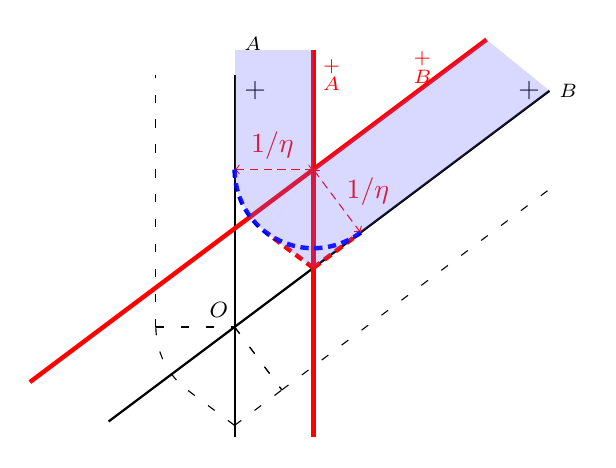
\begin{tikzpicture}[xscale=4,yscale=4]

\draw [thick] (1,0.65) -- (1,1.8);
\node [right] at (1, 1.9 ) {$\classifier_A$};
\node [right] at (1, 1.75 ) {$+$};

\draw [domain=0.6:2, thick] plot (\x, {3/4*\x+1/4});
\node [right] at (2, 1.75 ) {$\classifier_B$};
\node [left] at (2,1.75) {$+$};

\node [above] at (0.95, 1 ) {\footnotesize$O$};


\draw [domain=1+0.25*0.6:2, loosely dashed] plot (\x, {3/4*\x+1/4-5/16}); % 1/c = 1/4
\draw [loosely dashed] (1,1) -- (1+0.25*0.6,1-0.25*0.8);
\draw[loosely dashed] (0.75,1) -- (0.75,1.8);


\draw[loosely dashed] (1-0.25,1) arc (180:233.1:0.25);
\draw [loosely dashed] (1-0.25,1) -- (1,1);
\draw [loosely dashed] (1,11/16) -- (1-0.25*0.6,1-0.25*0.8);
% \node [left, font=\tiny] at (0.96,11/16) {\footnotesize$C$};
\draw [loosely dashed] (1,11/16) -- (1+0.25*0.6,1-0.25*0.8);
\draw [loosely dashed] (1,1) -- (1+0.25*0.6,1-0.25*0.8);



\draw [ultra thick,  red] (1.25,0.65) -- (1.25,1.88);
\node [right, red] at (1.25, 1.8 ) {$\classifier_A^{+}$};
\draw [<->, red, densely dashed] (1,1.5) -- (1+0.25,1.5);
\node [above, red] at (1+0.12, 1.5 ) {$1/\eta$};
\draw [domain=0.35:1.8, ultra thick, red] plot (\x, {3/4*\x+1/4+5/16});
\node [left, red] at (1.66, 3/4*1.68+1/4+5/16 ) {$\classifier_B^{+}$};

% \node [above, font=\tiny, red] at (1.23, 3/4*1.25+1/4+5/16 ) {\footnotesize$O'$};

\draw [<->, red, densely dashed] (1.25,3/4*1.25+1/4+5/16) -- (1.25+0.25*0.6,3/4*1.25+0.25*0.6*3/4+1/4 );
\node [right, red] at (1.25+0.125*0.6,3/4*1.25+3/4*0.125*0.6+7/16) {$1/\eta$};

\draw[red, densely dashed] (1,3/4*1.25+1/4+5/16) arc (180:233.1:0.25);

\draw [densely dashed, red, ultra thick] (1.25,1.25*0.75+0.25) -- (1.25-0.25*0.6,3/4*1.25+1/4+5/16-0.25*0.8);
% \node [below, font=\tiny, red] at (1.29,1.25*0.75+0.26) {\footnotesize$C'$};
\draw [densely dashed,red, ultra thick] (1.25,1.25*0.75+0.25) -- (1.25+0.25*0.6,3/4*1.25+0.25*0.6*3/4+1/4);


\draw[blue,densely dashed, ultra thick] (1,3/4*1.25+1/4+5/16) arc (180:360-53.1:0.25);


\fill [blue!60,nearly transparent]  
(1.8,6.4/4+5/16) --
(1.25,3/4*1.25+1/4+5/16) -- (1.25+0.25*0.6,3/4*1.25+0.25*0.6*3/4+1/4 ) --(2,7/4)-- cycle;

\fill [blue!60,nearly transparent]  (1,3/4*1.25+1/4+5/16) -- (1.25,3/4*1.25+1/4+5/16) -- (1.25,1.88) -- (1,1.88)-- cycle;

\fill [blue!60,nearly transparent] (1,3/4*1.25+1/4+5/16) -- (1.25,3/4*1.25+1/4+5/16) -- (1.25-0.25*0.6,3/4*1.25+0.25*0.6*3/4+1/4 )-- cycle;

\fill [blue!60,nearly transparent](1,3/4*1.25+1/4+5/16) coordinate (a) arc (180:233.1:0.25) -- cycle;

\fill [blue!60,nearly transparent] (1.25,3/4*1.25+1/4+5/16) -- (1.25+0.25*0.6,3/4*1.25+0.25*0.6*3/4+1/4 )--(1.25,4.75/4)--(1.25-0.25*0.6,3/4*1.25+0.25*0.6*3/4+1/4 )--cycle;

\end{tikzpicture}
\caption{An oversimplified intuition}
\label{fig: oversimplified intuition}
  \rule{0in}{1.2em}$^\dag$\scriptsize  This graph shows that under the same stringent tests $\classifier_A^+$ and $\classifier_B^+$, the fixed-order procedure that offers $\classifier_A^+$ first selects a larger set of potential qualified agents than the random-order procedure without disclosure and randomization probability $\frac12$.
  However, the optimal tests may not be the same for the two procedures. Hence, This intuition is oversimplified.
\end{figure}


We propose a new constructive argument to prove this result.
The idea is that fixing any feasible random order mechanism, we construct another feasible fixed-order mechanism that dominates the random-order mechanism.
We distinguish two cases.
In \cref{lem:feasible-informed-rand-distance cost}, we deal with the class of random-order mechanisms with disclosure.
In \cref{lem:feasible-uninformed-rand-distance cost}, we deal with the class of random-order mechanisms without disclosure.
This is a more involved case because the set of tests feasible for random-order mechanisms without disclosure is usually strictly larger.
It requires extra steps to construct the feasible fixed order mechanisms.

%---------------informed random order------------


\begin{lemma}\label{lem:feasible-informed-rand-distance cost}
 Suppose the  random-order mechanism  with disclosure $(\tilde\classifier_A,\tilde\classifier_B,q,\widetilde h_1)$ is feasible. 
 Then the two fixed-order mechanisms $(\tilde\classifier_A,\tilde\classifier_B,1)$ and $(\tilde\classifier_A,\tilde\classifier_B,0)$ are feasible and one of them is no worse than the  random-order mechanism with disclosure.
\end{lemma}



This is the simpler case because the set of tests feasible for random-order mechanisms with disclosure is the same as that for fixed-order mechanisms.
The challenge of this proof comes from that fixing the tests, neither of the two fixed-order mechanisms is directly comparable to any random-order mechanisms with disclosure.
This is because there is no nested structure between the set of types that can get selected by any of the two fixed-order mechanisms and that by any random-order mechanism with disclosure.
For example, see \cref{fig: same graph ran_informed fixed 2}. 
Our proof strategy is to introduce a mixed mechanism that randomizes over the two fixed-order mechanisms.
After that, we first apply a similar set inclusion argument to show that the mixed  mechanism dominates the random-order mechanism with disclosure.
And then we apply a probability argument to show that one of the fixed-order mechanisms used in the mixed mechanism dominates the mixed mechanism.




%---------------------------------------------------

Next, consider any random order mechanism without disclosure $(\tilde \classifier_A,\tilde \classifier_B, q, \varnothing)$. 
Let $\tilde O$ be the intersection point of the boundary lines of $ \tilde\classifier_A$ and $\tilde \classifier_B$. Let $\classifier_A'$ and $\classifier_B'$ be the tests that contain $\tilde O$ on their boundary lines and have the same normal vectors $\weights_A$ and $\weights_B$ as the half plane $\classifier_A$ and $\classifier_B$ respectively. 
%--------------------------random order uninformed---------------------------

\begin{lemma}\label{lem:feasible-uninformed-rand-distance cost}
 Suppose the random-order mechanism  without disclosure $(\tilde\classifier_A,\tilde\classifier_B,q,\nullset)$ is feasible.  
 Then two fixed order mechanisms $(\tilde\classifier_A,\classifier_B',1)$ and $(\classifier_A',\tilde\classifier_B,0)$ are also feasible.
 Moreover, one of these two fixed order mechanisms is no worse than the random-order mechanism without disclosure.
\end{lemma}

As we have eluded earlier, the set of tests feasible for random-order mechanisms without disclosure is usually larger. \cref{fig:shifted non-parallel random} provides an example.\footnote{One might hope that for those non-parallel tests, we can show that they are dominated by some parallel tests. 
However, this is not the case.
There is usually no way to rank the  tests that are feasible for random-order mechanisms without disclosure, even if we fix the randomization probability $q$.
 One example is \cref{fig:theta<30 random}. When the angle of the tests increase, the set of types being selected does not contain the set of types being selected under smaller angle of tests.
 Hence the constructive argument we propose here is required to compare any random-order mechanism without disclosure and any fixed-order mechanism.} 
Under the random order mechanism without disclosure $ (\tilde\classifier_A,\tilde \classifier_B,\frac12,\nullset)$, every selected agent uses a one-step strategy to pass both tests together. Hence the set of attributes being selected under this mechanism is the blue region and $\tilde\classifier_A\cap\tilde \classifier_B$.
Since the blue region is contained in the qualified region, this  mechanism is feasible.
However, since $\tilde\classifier_i,i\in\{A,B\}$ is not parallel to $\classifier_i,i\in\{A,B\}$, the corresponding fixed-order mechanisms are not feasible.
To see this, consider the unqualified attributes  $\orifeatures\in \widetilde h_B$ that are very closed to $\classifier_A$ but do not satisfy $\classifier_A$,  as shown in \cref{fig:shifted non-parallel random}.
Because the tests are non-parallel, we can always find such $\orifeatures$ so that its cost to pass $\widetilde h_A$ is less than one.
This implies that the fixed-order mechanism with $\widetilde h_B$ as the first test is not  feasible.
Similarly, we can argue that the fixed-order mechanism with $\widetilde h_A$ as the first test is not  feasible.

\begin{figure}[h]  
\centering 
\begin{tikzpicture}[xscale=4,yscale=4]

\draw [thick] (1,0.65) -- (1,1.8);
\node [right] at (1, 1.9 ) {$\classifier_A$};
\node [right] at (1, 1.75 ) {$+$};

\draw [domain=0.6:2, thick] plot (\x, {3/4*\x+1/4});
\node [right] at (2, 1.75 ) {$\classifier_B$};
\node [left] at (2,1.75) {$+$};


% \draw [ultra thick, red] (1.25,0.65) -- (1.25,1.88);
\node [right, red] at (1.26, 1.84 ) {$\widetilde\classifier_A$};
\draw [domain=1.17:1.29, ultra thick, red] plot (\x, {10*(\x-5/4)+3/2});
\draw [domain=0.5:1.76, ultra thick, red] plot (\x, {3.5/4*(\x-5/4)+3/2});
\node [left, red] at (1.6, 1.84 ) {$\widetilde\classifier_B$};

\node [left, font=\tiny] at (0.98, {3.5/4*(0.98-5/4)+3/2}) {\footnotesize$\orifeatures$};
\node [black] at (0.98, {3.5/4*(0.98-5/4)+3/2}) {\textbullet};

\draw[red, densely dashed] (1,3/4*1.25+1/4+5/16) arc (180:360-53.1:0.25);

\fill [blue!60,nearly transparent]  
((1.76, {3.5/4*(1.76-5/4)+3/2}) --
(1.25,3/4*1.25+1/4+5/16) -- (1.25+0.25*0.6,3/4*1.25+0.25*0.6*3/4+1/4 ) --(2,{3.5/4+1})-- cycle;

\fill [blue!60,nearly transparent]  (1,3/4*1.25+1/4+5/16) -- (1.25,3/4*1.25+1/4+5/16) -- (1.28, {10*(1.28-5/4)+3/2}) -- (1.04, {10*(1.28-5/4)+3/2})-- cycle;

\fill [blue!60,nearly transparent] (1,3/4*1.25+1/4+5/16) -- (1.25,3/4*1.25+1/4+5/16) -- (1.25+0.25*0.6,3/4*1.25+0.25*0.6*3/4+1/4 )-- cycle;

\fill [blue!60,nearly transparent](1,3/4*1.25+1/4+5/16) coordinate (a) arc (180:360-53.1:0.25) -- cycle;

\end{tikzpicture}
\caption{Feasible non-parallel tests for random-order mechanism without disclosure}
\label{fig:shifted non-parallel random}
\end{figure}

Here is a sketch of the proof for this lemma.
First we show that the two fixed order mechanisms $(\tilde\classifier_A,\classifier_B',1)$ and $(\classifier_A',\tilde\classifier_B,0)$ are feasible (See \cref{fig:construction uninformed random}). 
By combining one non-parallel test with one parallel test and a careful choice of the order of the tests, we make sure that no unqualified agent is selected under each of these fixed-order mechanisms.


Second, we use a similar argument to show dominance: we construct a mixed mechanism that randomizes over the two feasible fixed-order mechanisms $(\tilde\classifier_A,\classifier_B',1)$ and $(\classifier_A',\tilde\classifier_B,0)$, and then show that this mixed mechanism is weakly better than the random-order mechanism  without disclosure using the set inclusion argument. 
It follows naturally that  one of the two fixed-order mechanisms dominates the random-order mechanism without disclosure using a probability argument. All omitted proofs are in \cref{appendix: distance cost}.


\begin{figure}[h]  
\centering 
\begin{subfigure}{0.45\textwidth}
\begin{tikzpicture}[xscale=4,yscale=4]

\draw [thick] (1,0.78) -- (1,1.8);
\node [right] at (1, 1.9 ) {$\classifier_A$};
\node [right] at (1, 1.75 ) {$+$};

\draw [domain=0.7:2, thick] plot (\x, {3/4*\x+1/4});
\node [right] at (2, 1.75 ) {$\classifier_B$};
\node [left] at (2,1.75) {$+$};


\draw [ultra thick, blue] (1.25,0.78) -- (1.25,1.88);
\node [right, blue] at (1.26, 1.84 ) {$\classifier_A'$};
% \draw [domain=1.17:1.29, ultra thick, red] plot (\x, {10*(\x-5/4)+3/2});
\draw [domain=0.5:1.76, ultra thick, red] plot (\x, {3.5/4*(\x-5/4)+3/2});
\node [left, red] at (1.6, 1.84 ) {$\widetilde\classifier_B$};


\node [left, font=\tiny] at (0.98, {3.5/4*(0.98-5/4)+3/2}) {\footnotesize$\orifeatures$};
\node [black] at (0.98, {3.5/4*(0.98-5/4)+3/2}) {\textbullet};

\draw[red, densely dashed] (1,3/4*1.25+1/4+5/16) arc (180:360-53.1:0.25);

\fill [blue!60,nearly transparent]  
((1.76, {3.5/4*(1.76-5/4)+3/2}) --
(1.25,3/4*1.25+1/4+5/16) -- (1.25+0.25*0.6,3/4*1.25+0.25*0.6*3/4+1/4 ) --(2,{3.5/4+1})-- cycle;

\fill [blue!60,nearly transparent]  (1,3/4*1.25+1/4+5/16) -- (1.25,3/4*1.25+1/4+5/16) -- (1.25,1.88) -- (1,1.88)-- cycle;

\fill [blue!60,nearly transparent] (1,3/4*1.25+1/4+5/16) -- (1.25,3/4*1.25+1/4+5/16) -- (1.25+0.25*0.6,3/4*1.25+0.25*0.6*3/4+1/4 )-- cycle;

\fill [blue!60,nearly transparent](1,3/4*1.25+1/4+5/16) coordinate (a) arc (180:360-53.1:0.25) -- cycle;

\end{tikzpicture}
\end{subfigure}
\begin{subfigure}{0.45\textwidth}
\begin{tikzpicture}[xscale=4,yscale=4]

\draw [thick] (1,0.78) -- (1,1.8);
\node [right] at (1, 1.9 ) {$\classifier_A$};
\node [right] at (1, 1.75 ) {$+$};

\draw [domain=0.7:2, thick] plot (\x, {3/4*\x+1/4});
\node [right] at (2, 1.75 ) {$\classifier_B$};
\node [left] at (2,1.75) {$+$};


% \draw [ultra thick, red] (1.25,0.65) -- (1.25,1.88);
\node [right, red] at (1.26, 1.84 ) {$\widetilde\classifier_A$};
\draw [domain=1.18:1.29, ultra thick, red] plot (\x, {10*(\x-5/4)+3/2});
\draw [domain=0.5:1.76, ultra thick, blue] plot (\x, {3/4*(\x-5/4)+3/2});
\node [left, blue] at (1.6, 1.84 ) {$\classifier_B'$};


\node [left, font=\tiny] at (45/37, {3/4*(45/37-1)+1}) {\footnotesize$\features$};
\node [black] at (45/37, {3/4*(45/37-1)+1}) {\textbullet};

\draw[red, densely dashed] (1,3/4*1.25+1/4+5/16) arc (180:360-53.1:0.25);

\fill [blue!60,nearly transparent]  
((1.76, {3/4*(1.76-5/4)+3/2}) --
(1.25,3/4*1.25+1/4+5/16) -- (1.25+0.25*0.6,3/4*1.25+0.25*0.6*3/4+1/4 ) --(2,{3/4+1})-- cycle;

\fill [blue!60,nearly transparent]  (1,3/4*1.25+1/4+5/16) -- (1.25,3/4*1.25+1/4+5/16) -- (1.28, {10*(1.28-5/4)+3/2}) -- (1.04, {10*(1.28-5/4)+3/2})-- cycle;

\fill [blue!60,nearly transparent] (1,3/4*1.25+1/4+5/16) -- (1.25,3/4*1.25+1/4+5/16) -- (1.25+0.25*0.6,3/4*1.25+0.25*0.6*3/4+1/4 )-- cycle;

\fill [blue!60,nearly transparent](1,3/4*1.25+1/4+5/16) coordinate (a) arc (180:360-53.1:0.25) -- cycle;

\end{tikzpicture}
\end{subfigure}
\caption{Constructing feasible mixed mechanism for random-order mechanisms without disclosure}
\label{fig:construction uninformed random}
\end{figure}

\bigskip

%--------------------------------------------------


%---------------------------------------------------
\subsection{Cheap-talk}\label{subsec:cheap talk manipulation}
Third, we consider the case where the principal can tailor the tests to different types of agent, i.e., cheap-talk communication is allowed upfront.
We show that when cheap-talk communication is allowed,  a fixed-order sequential mechanism achieves the first best.

\begin{theorem}\label{thm: optimal max qualified cheap talk}
Suppose $M=\Featurespace$. 
% Consider the manipulation setting.
    % When the principal can only use linear tests, 
    For any distribution $\dist$, there exists a feasible fixed-order sequential mechanism that achieves the first best.
\end{theorem}

% The proof is constructive.
% We first introduce some useful notations. 
% Let $O$ be the intersection point of the boundary lines of $\classifier_A$ and $\classifier_B$. 
% Recall that  $\classifier_i^+, i\in \{A,B\} $ is a test obtained by shifting $\classifier_i$ along its normal vector $\weights_i$ by a distance of $1/\eta$.
% Denote  the intersection point of the boundary lines of $\classifier_A^+ $ and $\classifier_B^+ $ by $O^+$.
% Let $\widehat\classifier_A$ be the half plane obtained by rotating $\classifier_A^+ $ around point $O^+$ towards $\classifier_B^+ $ until the boundary line is exactly the angle bisector of $\classifier_A^+ $ and $\classifier_B^+$, which means the boundary of $\widehat \classifier_A$ goes through $O$.
% See \cref{fig:non-parallel stringent tests} for an illustration.

% Consider the fixed-order procedure $(\classifier_A^+,\classifier_B^+,1)$ and the fixed-order procedure $(\widehat\classifier_A,\classifier_B^+,1)$.
% Let $A$ be the intersection of boundaries of $\classifier_B$ and $\classifier_A^+$. Let $B$ be the intersection of boundaries of $\classifier_A$ and $\classifier_B^+$.
% The following two lemmas (partially) characterize the set of attributes that can get selected by these two fixed-order mechanisms. 


% \begin{lemma}\label{lem:gain non-parallel tests}
%  Under the fixed-order procedure $(\widehat\classifier_A,\classifier_B^+,1)$, we have the following:
%  \begin{itemize}
%      \item Each type in the triangle $\Updelta\text{OAB}$ has a profitable strategy to get selected.
%      \item No unqualified type has a strictly profitable strategy to get selected.
%  \end{itemize}
% \end{lemma}

% \begin{lemma}\label{lem:loss non-parallel tests}
%  Under the fixed-order procedure $(\classifier_A^+,\classifier_B^+,1)$, we have the following:
%  \begin{itemize}
%      \item Each type in $\classifier_A\cap\classifier_B\setminus \Updelta\text{OAB}$ has a profitable strategy to get selected.
%      \item Each type in the triangle $\Updelta\text{OAB}$ does not have a profitable strategy to get selected.
%      \item No unqualified type has a strictly profitable strategy to get selected.
%  \end{itemize}
% \end{lemma}

% \begin{figure}
% \centering
% \begin{tikzpicture}[xscale=5,yscale=5]

% \draw [thick] (-0.25,{-0.25/tan(30)}) -- (-0.25,0.8);
% \draw [domain=-0.25:0.8, thick] plot (\x, {tan(30)*\x-0.25/cos( 30)});
% \node [below] at (-0.25, {tan(30)*(-0.25)-0.25/cos( 30)} ) {$O$};

% \node [above] at (-0.25, 0.8 ) {$\classifier_B$};
% \node [above] at (0.8, {tan(30)*0.8-0.25/cos( 30)} ) {$\classifier_A$};
% \node [below] at (0.8, {tan(30)*0.8-0.25/cos( 30)} ) {$D$};
% % \draw [domain=-0.5:0.25, thick] plot (\x, {-tan(60)*(\x+0.25/cos( 30))});

% \draw [thick, blue] (0,0) -- (0,0.8);
% \draw [domain=-0.25:0.7, thick, blue] plot (\x, {tan(30)*\x});
% \node [above, blue] at (0, 0.8 ) {$\classifier_B^+$};
% \node [right, blue] at (0.7, {tan(30)*0.7} ) {$\classifier_A^+$};
% \draw [domain=-0.25:0, blue] plot (\x, {-tan(30)*\x-0.5*tan(30)});
% \node [right] at (0, {-0.5*tan(30)} ) {$B$};
% \node [left] at (-0.25, {tan(30)*0.25-0.5*tan(30)}) {$A$};

% \draw [domain=-0.25:0.4, thick, red] plot (\x, {tan(60)*\x});
% \node [above, red] at (0.4, {tan(60)*0.4} ) {$\widehat\classifier_A$};

% \draw [domain={0.25*sin(60)}:0.6, densely dashed, red] plot (\x, {tan(60)*\x-0.25/cos(60)});
% \node[above] at (0.6, {tan(60)*0.6-0.25/cos(60)}) {$E$};

% \draw [ red] (0,0) -- ({0.25*sin(60)},{-0.25*cos(60)});
% \draw[red] ({0.25*sin(60)},{-0.25*cos(60)}) arc (-30:-60:0.25);
% \draw [ red] (-0.25,0) -- (0,0);
% \draw [ red] (-0.25,0) -- (-0.25,{-0.25/tan(30)});
% \draw [ red] ({0.25*sin(30)},{-0.25*cos(30)}) -- (-0.25,{-0.25/tan(30)});
% \node[right] at  ({0.25*sin(30)},{-0.25*cos(30)}) {$C$};

% \node [right] at (-0.25,0.76 ) {$+$};
% \node [left] at (0.8, {tan(30)*0.8-0.25/cos( 30)}) {$+$};
% \node [left, red] at (0.4, {tan(60)*0.4}) {$+$};

% \fill [orange!60,nearly transparent]  (-0.25,{-0.25/tan(30)}) -- (-0.25,{-0.25*tan(30)}) -- (0,{-0.5*tan(30)}) -- cycle;
% \node [above, thick, orange] at (0, {-0.25/tan(30)}) {gain};

% \fill [purple!60,nearly transparent]  (0.6,{tan(60)*0.6-0.25/cos(60)}) -- ({(0.25/cos(60)-0.25/cos(30))/(tan(60)-tan(30))},{tan(30)*(0.25/cos(60)-0.25/cos(30))/(tan(60)-tan(30))-0.25/cos( 30)}) -- (0.8, {tan(30)*0.8-0.25/cos( 30)}) -- cycle;
% \node [above, thick, purple] at (0.68, {tan(30)*0.7}) {loss};

% \end{tikzpicture}
% \caption{Non-parallel stringent tests} \label{fig:non-parallel stringent tests}  
%  \rule{0in}{1.2em}$^\dag$\scriptsize Every type in the orange triangle $\Updelta \text{OAB}$ has a profitable strategy to be selected by the fixed-order procedure $(\widehat\classifier_A,\classifier_B^+,1)$ but has no profitable strategy to be selected by the fixed-order procedure $(\classifier_A^+,\classifier_B^+,1)$. In contrast, 
% every type in the purple triangle $\text{ECD}$ has no profitable strategy to be selected by the fixed-order procedure $(\widehat\classifier_A,\classifier_B^+,1)$ but has a profitable strategy to be selected by the fixed-order procedure $(\classifier_A^+,\classifier_B^+,1)$.
% \end{figure}

The proof is constructive.
We first introduce some useful notations. 
Let $O$ be the intersection point of the boundary lines of $\classifier_A$ and $\classifier_B$. 
Recall that  $\classifier_i^+, i\in \{A,B\} $ is a test obtained by shifting $\classifier_i$ along its normal vector $\weights_i$ by a distance of $1/\eta$.
Denote  the intersection point of the boundary lines of $\classifier_A^+ $ and $\classifier_B^+ $ by $O^+$.
Let $\widehat\classifier_A$ be the half plane obtained by rotating $\classifier_A^+ $ around point $O^+$ towards $\classifier_B^+ $ until the boundary line is exactly the angle bisector of $\classifier_A^+ $ and $\classifier_B^+$, which means the boundary of $\widehat \classifier_A$ goes through $O$.
% See \cref{fig:non-parallel stringent tests} for an illustration.

Consider the fixed-order procedure $(\classifier_A^+,\classifier_B^+,1)$ and the fixed-order procedure $(\classifier_A^+,\widehat\classifier_B,0)$.
Let $A$ be the intersection of boundaries of $\classifier_B$ and $\classifier_A^+$. Let $B$ be the intersection of 
boundaries of $\classifier_A$ and $\classifier_B^+$.
\cref{fig:cheap-talk} plots the set if qualified types that are selected by the two fixed-order procedures.
The fixed-order procedure $(\classifier_A^+,\classifier_B^+,1)$ that uses two shifted parallel tests select all qualified types except for those in 
the yellow triangle $\Updelta \text{OAB}$ (left panel).
However, any type in 
the yellow triangle $\Updelta \text{OAB}$ is selected by 
 the fixed-order procedure $(\classifier_A^+,\widehat\classifier_B,0)$ that uses one non-parallel test (right panel). Hence offering a menu of these two procedures can select all qualified types and no unqualified type.

\begin{figure}
    \centering
    \begin{subfigure}[b]{0.45\linewidth}
         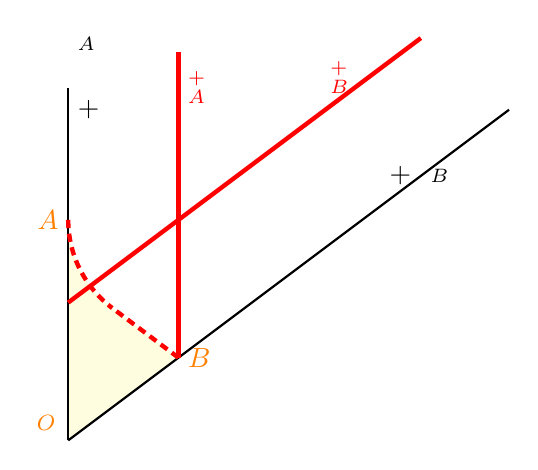
\begin{tikzpicture}[xscale=5.6,yscale=5.6]

\fill [yellow!50,nearly transparent]  (1,1.5) --(1,1)-- (1.25,1.25*0.75+0.25)--(1.25,1.5)  -- cycle;

\fill [white](1,3/4*1.25+1/4+5/16) coordinate (a) arc (180:233.1:0.25) -- cycle;
\fill [white]  (1,3/4*1.25+1/4+5/16) -- (1.25,3/4*1.25+1/4+5/16) -- (1.25-0.25*0.6,3/4*1.25+0.25*0.6*3/4+1/4 )-- cycle;
\fill [white] (1.25,3/4*1.25+1/4+5/16) -- (1.25+0.25*0.6,3/4*1.25+0.25*0.6*3/4+1/4 )--(1.25,4.75/4)--(1.25-0.25*0.6,3/4*1.25+0.25*0.6*3/4+1/4 )--cycle;

\draw [thick] (1,1) -- (1,1.8);
\node [right] at (1, 1.9 ) {$\classifier_A$};
\node [right] at (1, 1.75 ) {$+$};

\draw [domain=1:2, thick] plot (\x, {3/4*\x+1/4});
\node [right] at (1.8, 0.75*1.8+0.25 ) {$\classifier_B$};
\node [left] at (1.8, 0.75*1.8+0.25 ) {$+$};

\node [above, orange] at (0.95, 1 ) {\footnotesize$O$};


\draw [ultra thick,  red] (1.25,0.75*1.25+0.25) -- (1.25,1.88);
\node [right, red] at (1.25, 1.8 ) {$\classifier_A^{+}$};

\draw [domain=1:1.8, ultra thick, red] plot (\x, {3/4*\x+1/4+5/16});
\node [left, red] at (1.66, 3/4*1.68+1/4+5/16 ) {$\classifier_B^{+}$};

\node [left, orange] at (1,1.5) {$A$};
\node [right, orange] at (1.25,1.25*0.75+0.25) {$B$};



\draw[red, densely dashed, ultra thick] (1,3/4*1.25+1/4+5/16) arc (180:233.1:0.25);



\draw [densely dashed, red, ultra thick] (1.25,1.25*0.75+0.25) -- (1.25-0.25*0.6,3/4*1.25+1/4+5/16-0.25*0.8);


\end{tikzpicture}
    \end{subfigure}
    \begin{subfigure}[b]{0.45\linewidth}
        \begin{tikzpicture}[xscale=5.6,yscale=5.6]


\node [above] at (0.8, {tan(30)*0.8-0.25/cos( 30)} ) {$\classifier_B$};
\node [below, purple] at (0.8, {tan(30)*0.8-0.25/cos( 30)} ) {$D$};
% \draw [domain=-0.5:0.25, thick] plot (\x, {-tan(60)*(\x+0.25/cos( 30))});

\draw [domain={0.25*sin(60)}:0.5, densely dashed, red, ultra thick] plot (\x, {tan(60)*\x-0.25/cos(60)});
\node[above, purple] at (0.5, {tan(60)*0.5-0.25/cos(60)}) {$E$};


\draw[densely dashed, red, ultra thick] ({0.25*sin(60)},{-0.25*cos(60)}) arc (-30:-60:0.25);

\draw [thick] (-0.25,{-0.25/tan(30)}) -- (-0.25,0.45);
\draw [domain=-0.25:0.8, thick] plot (\x, {tan(30)*\x-0.25/cos( 30)});



\node [above] at (-0.25, 0.45) {$\classifier_A$};
\node [right] at (-0.25,0.4 ) {$+$};

\draw [domain=-0.25:0.25, ultra thick, red] plot (\x, {tan(60)*\x});
\node [above, red] at (0.25, {tan(60)*0.25} ) {$\widehat\classifier_B$};
\node [left, red] at (0.2, {tan(60)*0.2}) {$+$};

\draw [ultra thick, blue] (0,{-0.25/cos( 30)}) -- (0,0.45);
\node [above, blue] at (0, 0.45 ) {$\classifier_A^+$};

% \draw [densely dashed,  red] (-0.25,0) -- (-0.25,{-0.25/tan(30)});
% \draw [densely dashed,  red] ({0.25*sin(30)},{-0.25*cos(30)}) -- (-0.25,{-0.25/tan(30)});
\node[right, purple] at  ({0.25*sin(30)},{-0.25*cos(30)}) {$C$};


\node [left] at (0.8, {tan(30)*0.8-0.25/cos( 30)}) {$+$};


\fill [purple!60,nearly transparent]  (0.5,{tan(60)*0.5-0.25/cos(60)}) -- ({(0.25/cos(60)-0.25/cos(30))/(tan(60)-tan(30))},{tan(30)*(0.25/cos(60)-0.25/cos(30))/(tan(60)-tan(30))-0.25/cos( 30)}) -- (0.8, {tan(30)*0.8-0.25/cos( 30)}) -- cycle;
\node [above, thick, purple] at (0.6, {tan(30)*0.62}) {loss};

\end{tikzpicture}
    \end{subfigure}
    \caption{A menu of testing procedures that achieves the first best}
    \label{fig:cheap-talk}
\end{figure}

The formal proof is provided in \cref{appendix:cheap talk manipulation}. The key idea is that the union of the set of types selected by each fixed-order mechanism exactly coincides with the qualified region. 



% \begin{proof}[Proof of \cref{thm: optimal max qualified cheap talk}]
% The fixed-order mechanism is described as the following: 
% If the agent reports a type in the triangle $\Updelta \text{OAB}\subset \classifier_A\cap\classifier_B$, then the principal announces the fixed-order mechanism $(\tilde\classifier_A,\classifier_B^+,1)$.
%  If the agent reports a type in $ \classifier_A\cap\classifier_B\setminus \Updelta \text{OAB}$, then the principal announces the fixed-order mechanism $(\classifier_A^+,\classifier_B^+,1)$. 
%  If the agent reports a type that is not in $ \classifier_A\cap\classifier_B$, then the principal randomly announces either $(\tilde\classifier_A,\classifier_B^+,1)$ or $(\classifier_A^+,\classifier_B^+,1)$.

% First, we show that this fixed-order mechanism is feasible. 
% By \cref{lem:gain non-parallel tests} and \cref{lem:loss non-parallel tests}, no unqualified type has a profitable strategy to get selected under either $(\tilde\classifier_A,\classifier_B^+,1)$ or $(\classifier_A^+,\classifier_B^+,1)$.
% Hence no unqualified type has a profitable strategy to get selected regardless of the reporting strategy.

% Next we show that under this fixed-order mechanism, every qualified agent is selected.
% By \cref{lem:gain non-parallel tests} and \cref{lem:loss non-parallel tests}, each type in the triangle $\Updelta \text{OAB}$ has a profitable strategy to get selected by the fixed-order mechanism $(\tilde\classifier_A,\classifier_B^+,1)$ but not in the fixed-order mechanism $(\classifier_A^+,\classifier_B^+,1)$.
% Hence each type in the triangle $\Updelta \text{OAB}$ has incentive to truthfully report his type and gets selected. Again, by \cref{lem:loss non-parallel tests}, each type in $\classifier_A\cap\classifier_B\setminus \Updelta\text{OAB}$ has a profitable strategy to get selected by the fixed-order mechanism $(\classifier_A^+,\classifier_B^+,1)$ if he reports truthfully.\footnote{Here some types in $\classifier_A\cap\classifier_B\setminus \Updelta\text{OAB}$ might have incentive to misreport if they can get selected by the fixed-order mechanism $(\tilde\classifier_A,\classifier_B^+,1)$ with a lower cost. }
% \end{proof}

%-----------------------------------------
\bigskip



\subsection{Comparison to simultaneous mechanisms}\label{subsec: simultaneous manipulation}
Second, we ask whether conducting both tests together could improve upon conducting one test at a time.
In other words, we ask whether simultaneous mechanisms could work better than sequential mechanisms.
\citet{zigzag} have studied the comparison between fixed-order mechanisms and simultaneous mechanisms under the manipulation setting and the same cost function.
 We state a similar result and in \cref{thm:opt_manipulation} we generalize it to a broader class of cost functions.\footnote{We view our \cref{lem:fix-simultaneous-distance cost} as a correction of Theorem 4.4 in \citet{zigzag}. 
The main issue there is that they first show the optimal tests for both simultaneous mechanisms and fixed order mechanisms must use shifted parallel tests.
\cref{fig:cheap-talk} serves as a counterexample to illustrate a fixed-order mechanism that uses shifted non-parallel tests could dominate one that uses shifted parallel tests under some distribution.
}
%------------------------------------
\begin{proposition}\label{lem:fix-simultaneous-distance cost}
% Consider the manipulation setting and additive Euclidean distance cost.
    The optimal fixed-order mechanism dominates the optimal simultaneous mechanism. Moreover, it uses stringent tests $\widetilde\classifier_A, \widetilde\classifier_B$, i.e., $\widetilde\classifier_A\cap \widetilde\classifier_B \subsetneq \classifier_A\cap \classifier_B$.
\end{proposition}

% \cref{lem:fix-simultaneous-distance cost} This result is implied by \cref{thm:opt_manipulation}.
The proof idea is to first show that the optimal simultaneous mechanism uses shifted tests that are parallel to the principal's true criteria.
% This is because shifted non-parallel tests are either not feasible or not optimal (See \cref{fig:non-parallel tests not optimal}).
And then we show that one fixed-order mechanism that uses the same tests weakly increases the chance of selecting an agent. 


%--------------------------------------------
To understand this proposition, suppose the test $\classifier_{A} \cap \classifier_{B}$ is used in the simultaneous mechanism. 
This implies that any agent with true attributes $\orifeatures\in \classifier_{A} \cap \classifier_{B}$
will not manipulate and will be selected. In addition, agents with true
attributes $\orifeatures\notin \classifier_{A} \cap \classifier_{B}$ will be selected only if they pay a
 cost to adopt attributes that are in the qualified region. Since
the benefit of doing so (i.e., getting selected) is 1, only those with cost
no greater than 1 will be willing to do so. The set of candidates who are
willing to do such preparation is 
\[
\manipulation=\left\{ \orifeatures\notin h_{A}\cap h_{B}:\min_{\features\in h_{A}\cap
h_{B}}\onecost(\orifeatures,\features)\leq 1\right\} \text{.}
\]%
This set $\manipulation$ comprises all points whose distance to either the two edges of
the qualified region $h_{A}\cap h_{B}$ is no greater than 1.

The simultaneous mechanism that uses tests $%
h_{A}\cap h_{B}$ selects some unqualified agents, so does not satisfy
the principal's objective. In order not to select any unqualified agents,
the principal must choose a more stringent test. For example,   $h_{A}^{+}\cap h_{B}^{+}$, where $h_{i}^{+}$ is
obtained by a parallel shift of $h_{i}$ by a distance of $1/\eta$. It turns out $h_{A}^{+}\cap
h_{B}^{+}$ is the optimal simultaneous mechanism.
This is because shifted non-parallel tests are either not feasible or not optimal under any simultaneous procedure (See \cref{fig:non-parallel tests not optimal}).


\begin{figure}
\centering 
    \begin{subfigure}{0.45\textwidth}
\centering 
\begin{tikzpicture}[xscale=4,yscale=4]

\draw [thick] (1,0.65) -- (1,1.8);
\node [right] at (1, 1.9 ) {$\classifier_A$};
\node [right] at (1, 1.75 ) {$+$};

\draw [domain=0.6:2, thick] plot (\x, {3/4*\x+1/4});
\node [right] at (2, 1.75 ) {$\classifier_B$};
\node [left] at (2,1.75) {$+$};


\draw [ultra thick, red] (1.25,0.65) -- (1.25,1.88);
\node [right, red] at (1.25, 1.8 ) {$\classifier_A^{+}$};
% \draw [<->, red, densely dashed] (1,1.5) -- (1+0.25,1.5);
% \node [above, red] at (1+0.125, 1.5 ) {$1$};
\draw [domain=0.35:1.8, ultra thick, red] plot (\x, {2.5/4*(\x-5/4)+3/2});
\node [left, red] at (1.64, 3/4*1.66+1/4+5/16 ) {$\widehat\classifier_B$};


\draw[red, densely dashed] (1,3/4*1.25+1/4+5/16) arc (180:360-53.1:0.25);

\fill [blue!60,nearly transparent]  
(1.8,{2.5/4*(1.8-5/4)+3/2}) --
(1.25,3/4*1.25+1/4+5/16) -- (1.25+0.25*0.6,3/4*1.25+0.25*0.6*3/4+1/4 ) --(2,6.5/4)-- cycle;

\fill [blue!60,nearly transparent]  (1,3/4*1.25+1/4+5/16) -- (1.25,3/4*1.25+1/4+5/16) -- (1.25,1.88) -- (1,1.88)-- cycle;

\fill [blue!60,nearly transparent] (1,3/4*1.25+1/4+5/16) -- (1.25,3/4*1.25+1/4+5/16) -- (1.25+0.25*0.6,3/4*1.25+0.25*0.6*3/4+1/4 )-- cycle;

\fill [blue!60,nearly transparent](1,3/4*1.25+1/4+5/16) coordinate (a) arc (180:360-53.1:0.25) -- cycle;

\end{tikzpicture}
\caption{Not feasible non-parallel tests}
\end{subfigure}
\begin{subfigure}{0.45\textwidth} 
\centering 
\begin{tikzpicture}[xscale=4,yscale=4]

\draw [thick] (1,0.65) -- (1,1.8);
\node [right] at (1, 1.9 ) {$\classifier_A$};
\node [right] at (1, 1.75 ) {$+$};

\draw [domain=0.6:2, thick] plot (\x, {3/4*\x+1/4});
\node [right] at (2, 1.75 ) {$\classifier_B$};
\node [left] at (2,1.75) {$+$};


\draw [ultra thick, red] (1.25,0.65) -- (1.25,1.88);
\node [right, red] at (1.25, 1.8 ) {$\classifier_A^{+}$};
% \draw [<->, red, densely dashed] (1,1.5) -- (1+0.25,1.5);
% \node [above, red] at (1+0.125, 1.5 ) {$1$};
\draw [domain=0.35:1.76, ultra thick, red] plot (\x, {3.5/4*(\x-5/4)+3/2});
\node [left, red] at (1.63, {3.5/4*(1.65-5/4)+3/2} ) {$\widetilde \classifier_B$};

% \draw [<->, red, densely dashed] (1.25,3/4*1.25+1/4+5/16) -- (1.25+0.25*0.6,3/4*1.25+0.25*0.6*3/4+1/4 );
% \node [right, red] at (1.25+0.125*0.6,3/4*1.25+3/4*0.125*0.6+7/16) {$1$};


\draw[red, densely dashed] (1,3/4*1.25+1/4+5/16) arc (180:360-53.1:0.25);

\fill [blue!60,nearly transparent]  
((1.76, {3.5/4*(1.76-5/4)+3/2}) --
(1.25,3/4*1.25+1/4+5/16) -- (1.25+0.25*0.6,3/4*1.25+0.25*0.6*3/4+1/4 ) --(2,{3.5/4+1})-- cycle;

\fill [blue!60,nearly transparent]  (1,3/4*1.25+1/4+5/16) -- (1.25,3/4*1.25+1/4+5/16) -- (1.25,1.88) -- (1,1.88)-- cycle;

\fill [blue!60,nearly transparent] (1,3/4*1.25+1/4+5/16) -- (1.25,3/4*1.25+1/4+5/16) -- (1.25+0.25*0.6,3/4*1.25+0.25*0.6*3/4+1/4 )-- cycle;

\fill [blue!60,nearly transparent](1,3/4*1.25+1/4+5/16) coordinate (a) arc (180:360-53.1:0.25) -- cycle;

\end{tikzpicture}
 \caption{Not optimal non-parallel tests}  
 \end{subfigure}
 \caption{Shifted non-parallel tests are not optimal}
 \label{fig:non-parallel tests not optimal}
\end{figure}

Suppose now the principal uses a fixed-order sequential mechanism that offers test $h_{A}$ at the first stage, and (2) among those
selected in (1), those who can pass test $h_{B}$ will be eventually
selected. We can characterize the set of attributes that get selected under such a fixed-order mechanism (\cref{fig: zig zag}) using the geometric intuition offered in \cref{subsec:example}.

In order not to select any unqualified agent, the principal needs to choose
more stringent tests instead of $h_{A}$ and $h_{B}$. One obvious candidate is the same stringent tests used in the optimal simultaneous mechanism: $%
h_{A}^{+}$ and $h_{B}^{+}$.
It remains to check that all agents selected by the fixed-order sequential mechanism are qualified under tests $%
h_{A}^{+}$ and $h_{B}^{+}$.
It turns out that this is indeed the case here (see \cref{fig: oversimplified intuition}).\footnote{In general, there are tests that are feasible under simultaneous mechanisms but are not feasible under fixed-order sequential mechanisms.}


\citet{zigzag} showed that the optimal simultaneous mechanism  $h_{A}^{+}\cap h_{B}^{+}$ is dominated by the fixed-order sequential mechanism $%
h_{A}^{+}$ and $h_{B}^{+}$; however, there is an error in the proof of their main result (Theorem 4.4), which we correct here. 
Observe that by using the fixed-order sequential mechanism $%
h_{A}^{+}$ and $h_{B}^{+}$, the principal selects more agents than
by using the simultaneous mechanism $h_{A}^{+}\cap h_{B}^{+}$. This is
because the fixed-order sequential mechanism enables agents to use two-step
strategies, which are cheaper (sometimes strictly) than the best one-step
strategy. 
We conclude that the optimal simultaneous mechanism is dominated by some sequential mechanisms. 
Moreover, in order to avoid unqualified agents, any feasible sequential mechanisms must use stringent tests.